\documentclass[12pt]{article}

% import packages
\usepackage[utf8]{inputenc}
\usepackage{float}
\usepackage{subfloat}
\usepackage{subfig}
\usepackage{amsmath}
\usepackage[toc,page]{appendix}
\usepackage{caption}
\usepackage{graphicx}
\usepackage{hyperref}
\usepackage[left=1in,top=0.75in,right=1in,bottom=0.75in]{geometry}

\graphicspath{ {./images} }
% hyperref setup
\hypersetup{
	colorlinks=true,
	linkcolor=blue,
	filecolor=blue,      
	urlcolor=blue,
	citecolor=blue,
	pdftitle={Stirling engine lab report},
	pdfpagemode=FullScreen,
}

% titlepage	
\title{\textbf{Stirling engine lab report}}
\author{Callum Stephenson, css47, GRP173, Trinity}
\date{}

\begin{document}
    \begin{titlepage}
        \thispagestyle{empty}
        \maketitle
    \end{titlepage}
    \tableofcontents
    \section{Abstract}
    Within this report, a real stirling engine is captured through use of a Raspberry Pi and compared to theoretical efficiencies. It was found that theoretical efficiency decreases
    with input power, but the output power increased. Although, all of the input power produce relatively low efficiency compared with modern engines. There is also a significance
    placed on how the data is handled, and approximations (such as small angle) used to make the data easier to handle. Given more time, developing a program which calculates
    the volume to completeness would be useful as such a calculation is trivial to a computer. 
    \section{Introduction}
        The stirling engine is a 4 stage cycle engine as illustrated in figure \ref{stirlingcycle}.
        \begin{figure}[H]
            \captionsetup{labelfont=bf}
            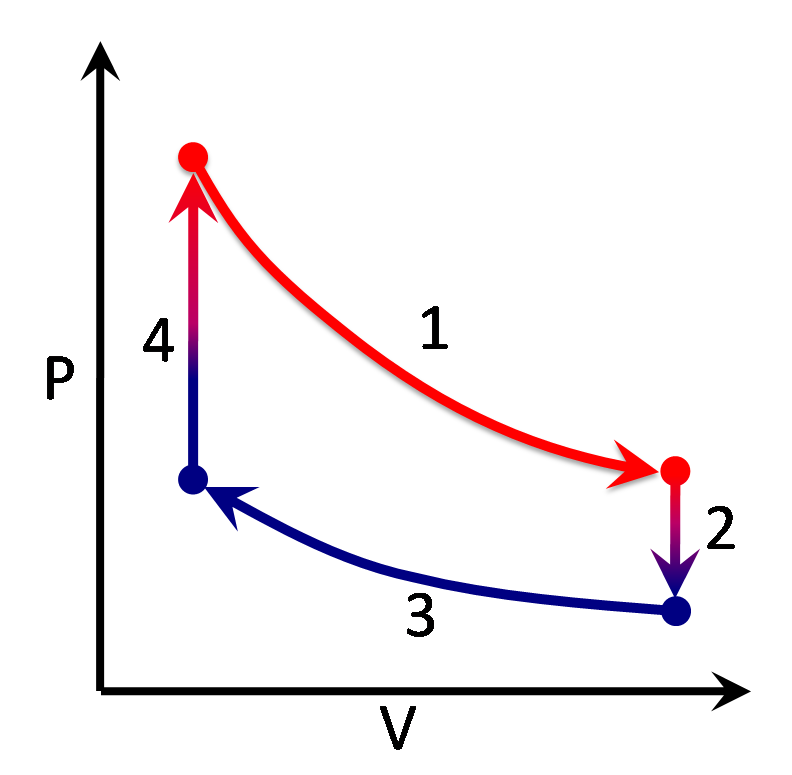
\includegraphics[width=20pc]{stirlingcycle.png}
            \caption{p-v diagram showing the ideal stirling cycle}\label{stirlingcycle}
        \end{figure}
        From 1 to 2, the gas is expands due to heating from the $T_{hot}$ source, pushes the work piston up extracting work. From 2 to 3, the displacer moves down and the hot gas
        begins to cool at constant volume, resulting in a reduction of pressure. From 3 to 4, the gas cools and contracts giving up heat to the sink at $T_{cold}$, and both pistons
        move toward the centre of the cylinder. From 4 to 1, the displacer piston is moving upwards and the gas it heating, the volume of the gas remains constant but increases in pressure.
        The p-v diagram is very useful in calculating the cycle power as the contour integral around one cycle is the work done. $\oint_{rev}p \delta v = W_x$ - we can compare this area 
        to our actual cycle in order to calculate the efficiency of a real device.
    \section{Methodology}
        We are able to represent the volume of gas as the sum of the volume of the large cylinder and $\pi r_{smallcyl}^2x$ where $x = x_{total} - x'$. We have a triangular
        mechanism holding the small piston to the flywheel represented by the two lengths $L_1$ and $L_2$. Thus, x' can be represented as $L_1 \cos (\pi - \phi) + L_2 \cos(\theta)$.
        Where theta is the angle between L2 and the piston, and pi - phi is the angle between L1 and the flywheel. The maximum theta value obtainable through small angle substitution
        of $\cos = 1$ (sufficiently small to be accurate) is $\theta = \arcsin(\frac{L_1}{L_2})$. The ratio  between $L_1$ and $L_2$ is 0.205, which would give a theta max of 0.206 (approximately $\sin \theta = \theta$)
        Using the approximation, at $\theta_{max}$, the value of x is 12.6 mm. Using the true value, 13.9mm which gives a difference of 10\% which is a reasonable approximation. Using
        the second approximation, the difference is only 0.5\% at the maximum value of theta - hence this is the more useful approximation for our scenario. \\ \\

        For a human to calculate the energy per cycle, they can count the squares in the cycle. This is about 5 for the first heater cycle. That would give an energy/cycle value
        of 0.025 J. This occured in 0.2 s, hence the power is 0.125 W. This leaves $\eta = \frac{0.125}{33} = 0.37 \%$. This works as we know that $w_x = \oint_{rev} p \delta v$, so this
        is why this estimation works to quickly calculate the power. It is hard to make a computer "sum the squares" within a graph - so it is easier to use a numerical method using
        the cross product of vectors.
    \section{Results}
        Both the ideal and real cycle are much smaller than the carnot cycle, and therefore less efficient (as seen in figure \ref{cycle1}). The carnot efficiencies are 0.33, 0.46, and 0.54
        for 1, 2, and 3 heaters respectively. The ideal stirling energy output is given by $E = m.(T_h - T_c).R.\ln(CR)$ where CR is 1.055. The ideal stirling cycles are 0.31 J, 0.58 J and 0.81 J respectively. Ideal
        efficiencies are 0.9\%, 0.87\%, and 0.81\% respectively. The real efficiencies are 0.325 \%, 0.34\%, and 0.35\% respectively. 
        The actual efficiency is greatly lower than the carnot efficiency or the ideal stirling efficiencies. As the power input is increased, real efficiency increases but theoretical efficiency
        decreases. However, running at higher input power means higher output power, and even though the efficiency may decrease there will be an improved output power.
        \begin{figure}[H]
            \captionsetup{labelfont=bf}
            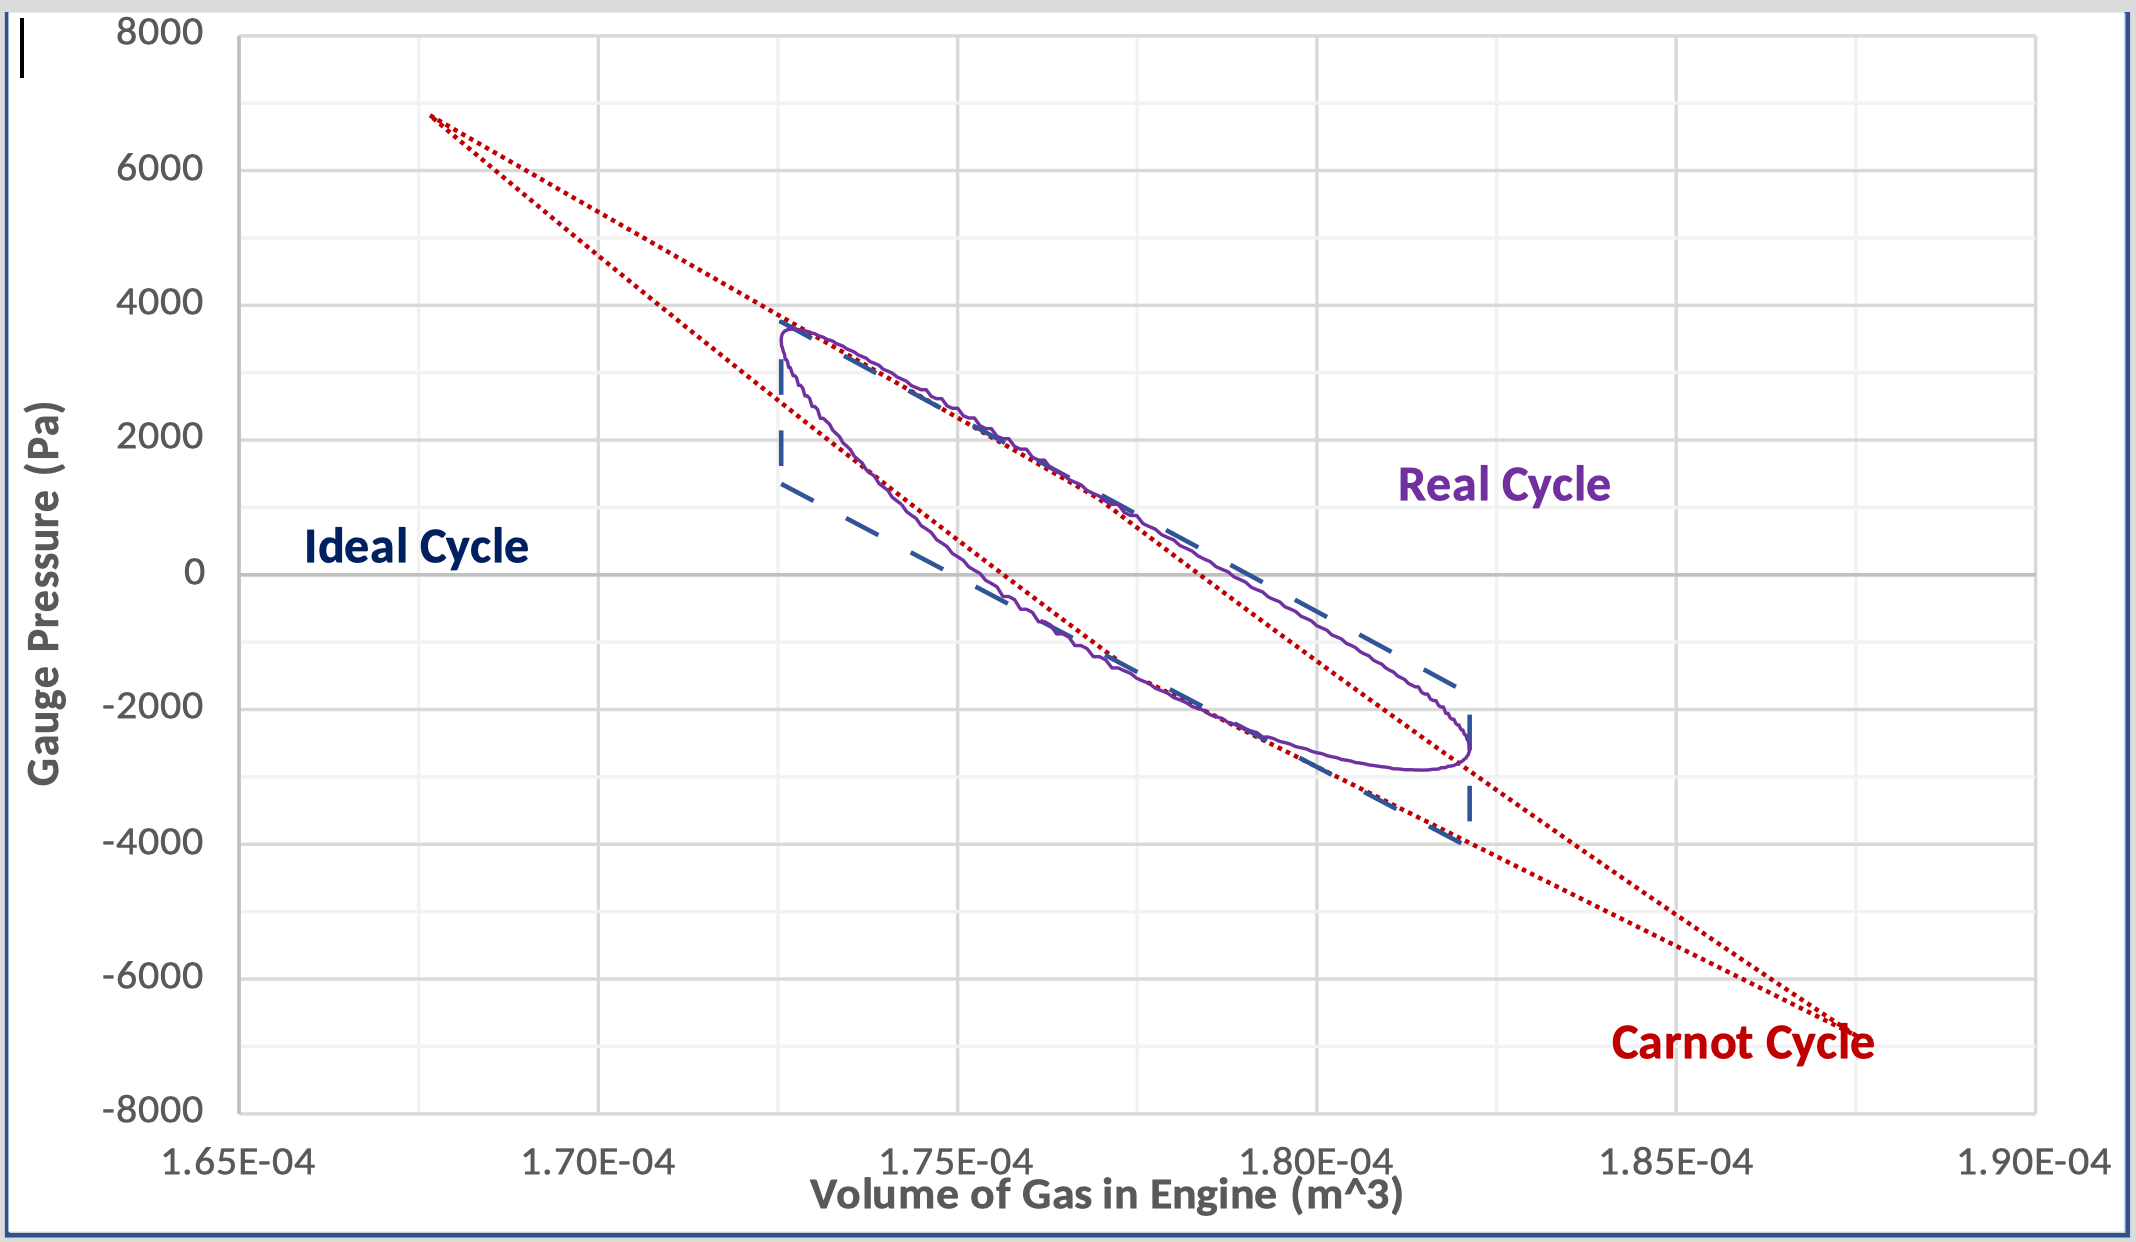
\includegraphics[width=40pc]{cycle1.png}
            \caption{p-v diagram showing the stirling cycle with 1 heater}\label{cycle1}
        \end{figure}
        \begin{figure}[H]
            \captionsetup{labelfont=bf}
            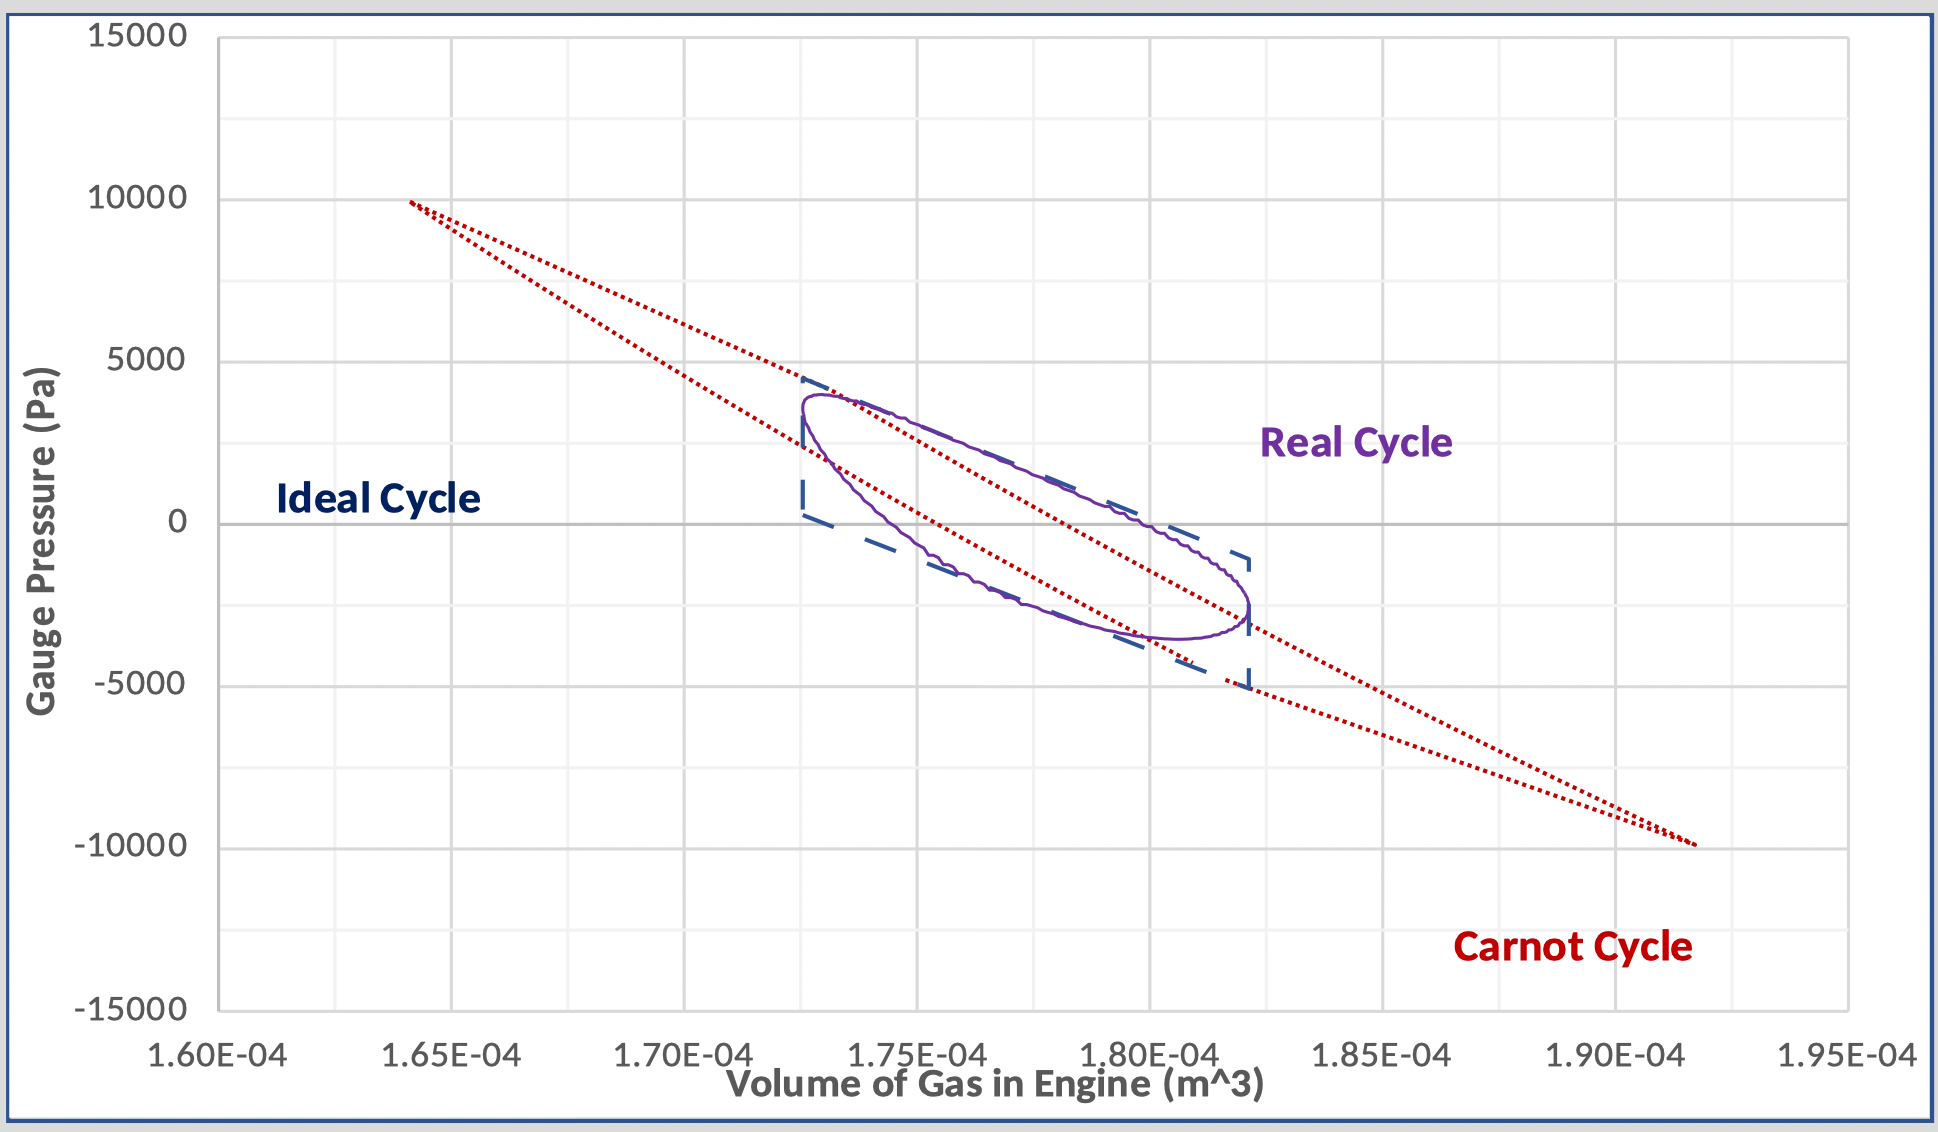
\includegraphics[width=40pc]{cycle2.png}
            \caption{p-v diagram showing the stirling cycle with 2 heaters}\label{cycle2}
        \end{figure}
        \begin{figure}[H]
            \captionsetup{labelfont=bf}
            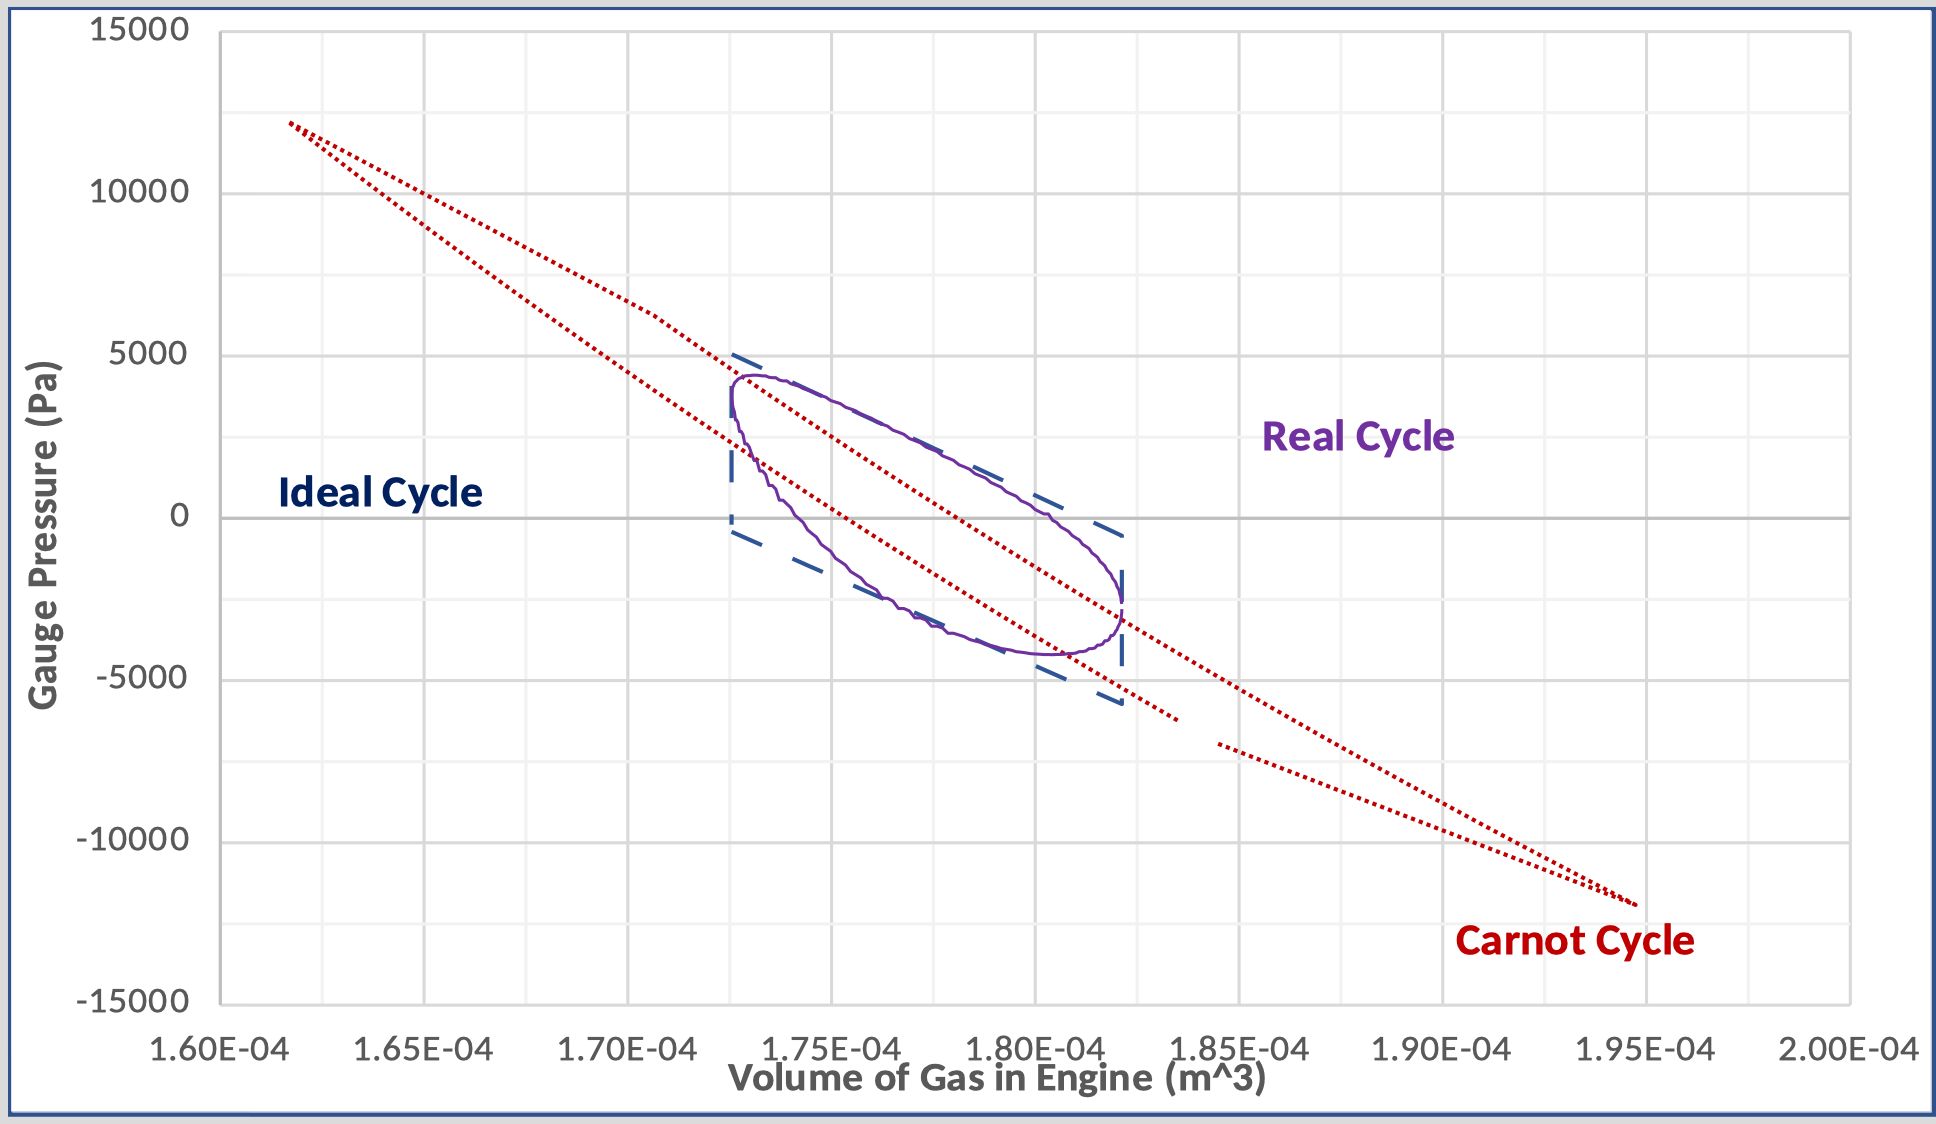
\includegraphics[width=40pc]{cycle3.png}
            \caption{p-v diagram showing the stirling cycle with 3 heaters}\label{cycle3}
        \end{figure}
        Comparing the cycles, there is a greater range of pressurs and volumes when using higher input, which you would expect as each cycle has more heat input and more work output.
        Greater ranges in these leads to greater variance in thermodynamic states. 
    \section{Conclusion}
        By using suitable approximation and using computer logging software, it was possible to calculate the real efficiency of a stirling engine. This allows for comparison
        to the ideal stirling cycle and the carnot efficiency. It is also demonstrated how useful p-v diagrams can be in extracing information about a cycle. If this experiment
        were to be run again, a parallel T-s diagram would be great in order to see the heat transfer in and out of the system. T-s diagrams are more intuitive to see the inputs
        and outputs of a system as work or heat. As a sidenote, computer logging techniques are extremely important in industry in order to regulate processes within a plant.
        It is important to accurately know the state of your system in order to input it into a PID controller or another controller along those lines in order to feed back
        into the system to improve conditions and efficiency. Though, given more time - it would be easier to implement a proper calculation of the angle rather than an approximation,
        as for a computer running this calculation is trivial - and the accuracy sacrificed is unnecessary in this stage. The theoretical efficiency of the stirling engine reduces
        with higher input power, however if a certain output power is required - then the efficiency may not matter as much as the ability of the system to output the required power.
         Either way, this cycle is inefficient compared to modern gas power plants or modern petrol or diesel engines. It also has a relatively high power/weight ratio, which makes
         it unsuitable for vehicles. 
    \end{document}